\documentclass{beamer}
\usepackage[utf8]{inputenc}
\usepackage{hyperref}
\usepackage{multicol}
\usepackage{hyperref}
\usepackage{graphicx}
\usepackage{booktabs}
\hypersetup{
    colorlinks=true,
    urlcolor={blue!40!black},
    linkcolor={red!50!black}
}

\inputencoding{utf8}

\mode<presentation> {
    \usetheme{Madrid}
}

\title[Introducciòn]{Introducci\'on al curso de Analisis, dise\~{n}o y fabricaci\'on de sistemas}
\author{Prof. Ernesto Rodriguez}
\institute{
    Universidad del Itsmo \\
    \medskip \textit{erodriguez@unis.edu.gt}
}

\date[\today]{}

\begin{document}

\begin{frame}
\titlepage
\end{frame}

\begin{frame}
\frametitle{Primero, un chiste...}
\begin{center}
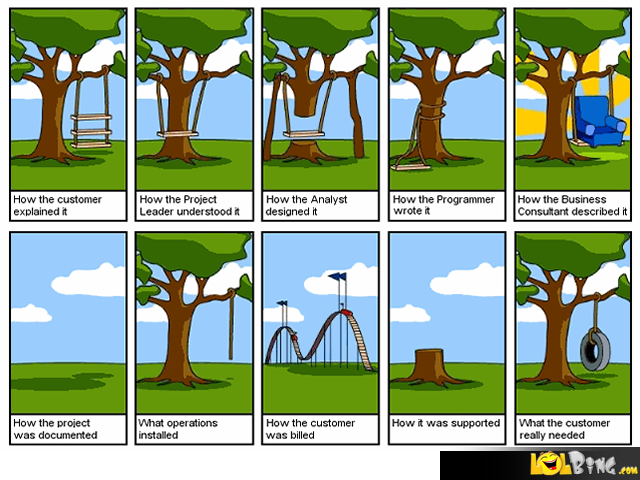
\includegraphics[width=10cm]{software-engineering-explained.png}
\end{center}
\end{frame}

\begin{frame}
    \frametitle{Composici\'on del curso}
    \begin{tabular}{|c|p{3.8cm}|c|c|}
        \hline
        \bf{Art\'iculo} & \bf{Detalles} & \bf{Valor unitario} & \bf{Valor total} \\
        \hline
        Hoja de trabajo & 4 hojas de trabajo para poner en practica el material estudiado en clase & 7.5\% & 30\% \\
        \hline
        Parcial teorico & El 1er y 3er examen parcial seran teoricos. & 10\% & 10\% \\
        \hline
        Parcial practico & El 2do examen parcial sera una entrega intermedia del proyecto final. & 10\% & 10\% \\
        \hline
        Examen final & 50\% teorico y 50\% entrega final del proyecto. & 40\% & 40\% \\
        \hline
        
    \end{tabular}
\end{frame}

\begin{frame}
\frametitle{Herramientas y Recursos}
A excepci\'on de Latex, Git y Github, el estudiante tiene la libertad de
utilizar las herramientas que el desea. Esto incluye: lenguaje de programaci\'on,
editor de codigo, software para diagramas, herramientas de documentaci\'on, ect.

\begin{multicols*}{2}
    {\bf Herramientas} \\
\begin{itemize}
    \item \href{https://code.visualstudio.com/}{Visual Studio Code}
    \item \href{https://git-scm.com/}{Git}
    \item \href{https://github.com/}{Github}
    \item \href{https://www.latex-project.org/}{Latex}
    \item \href{https://dotnet.github.io/}{.Net Core}
    \item \href{https://wiki.gnome.org/Apps/Dia}{Dia (Herramienta para diagramas)}

\end{itemize}
\columnbreak
{\bf Recursos}
\begin{itemize}
    \item Latex Wiki \cite{Latex}
    \item Git tutorial \cite{GitTutorial}
    \item .Net Core Guide \cite{DotNetGuide}
    \item XML Comments \cite{XmlDoc}
\end{itemize}
\end{multicols*}
\end{frame}

\begin{frame}
\frametitle{Referencias}
\bibliography{../../Referencias/referencias}
\bibliographystyle{plain}
\end{frame}

\end{document}